\chapter{Goals}
Our goal is to develop a graphical editor for music generation. With it's help it will be possible to create patches, test their output in a simulation and produce a netlist to generate that sound on a FPGA. A patch can be build with different components like wave generators and filters. In order to create specific sounds, the components have to be connected. The exported netlist can be put on a FPGA so the user of the synthesizer (e.g. a musician) can connect a MIDI device or specific sensors to the FPGA to modify input values at runtime. 

To describe the functions, which we want to develop, in detail, we provide use case diagrams.

\section{Editor for the designer}

	\begin{figure}[!h]
		\centering
			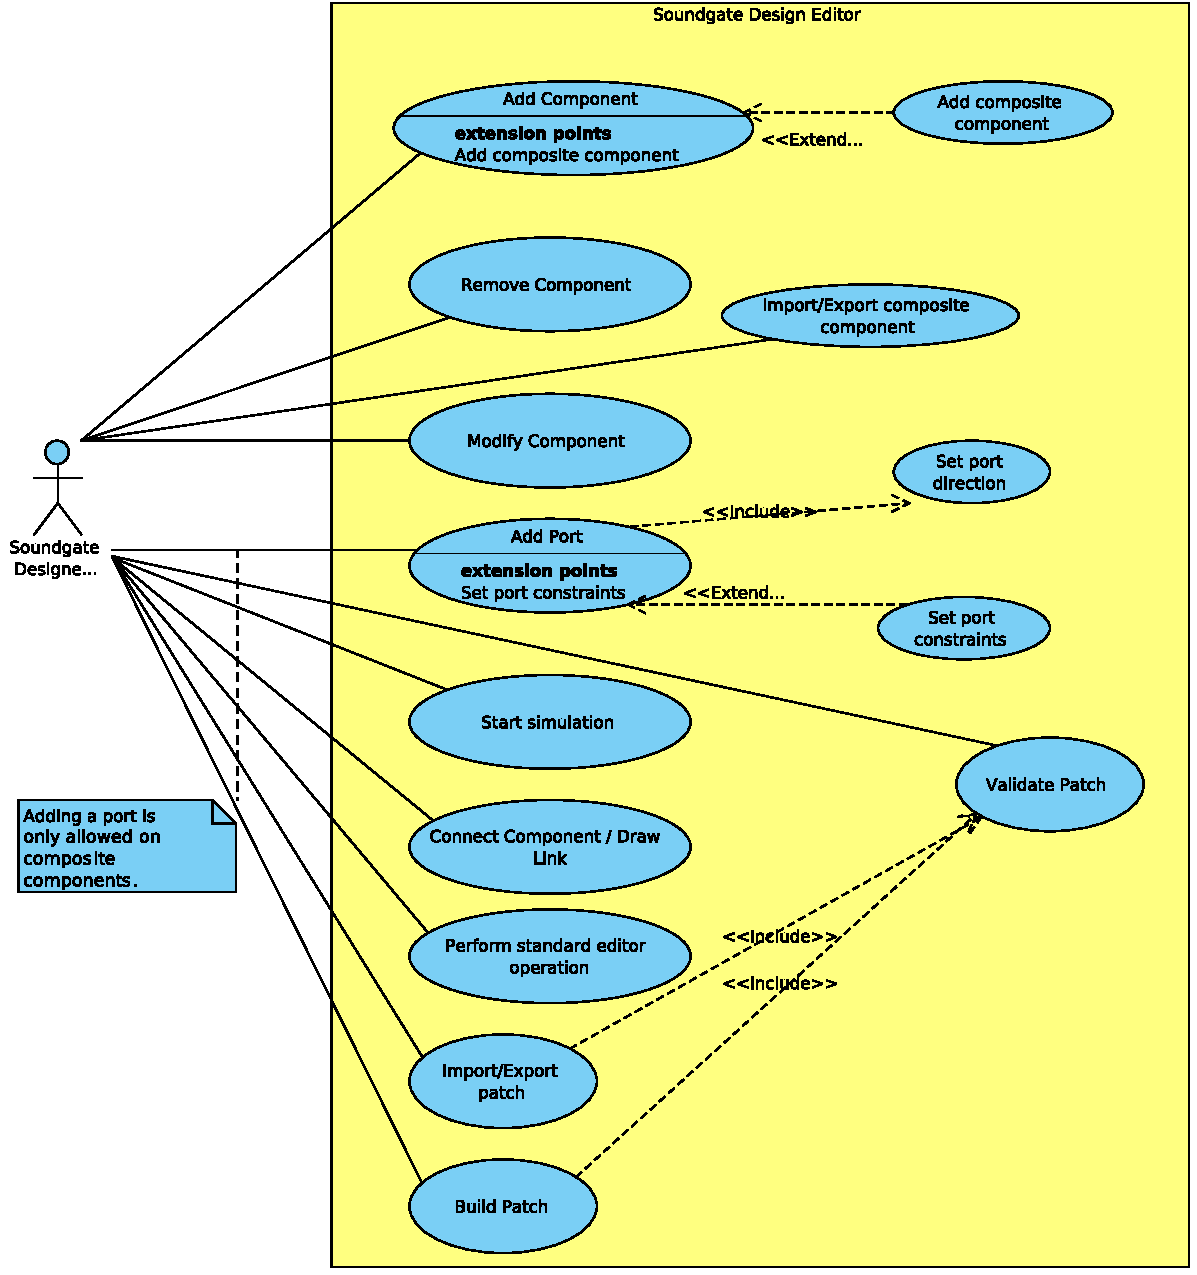
\includegraphics[width=0.93\textwidth]{images/Soundgate_Designer.pdf}
		\caption{Use case diagram of the soundgate designer (editor)}
		\label{fig:Soundgate_Designer}
	\end{figure}
	
The designer can add components to the patch and remove them from the patch. He can connect components by drawing links between their ports. A component can be an atomic component like a sound generator, filter etc. The atomic components are stored within XML-libraries. Some of these components have static properties, which the designer can modify (e.g. the value of a constant-block). The other kind of components are composite components. The designer can add a composite component to the patch and fill it on his own with other components and links between them. He can add ports to a composite component and define their direction and constraints. We want to make it possible to export finished composite components as XML-files and to import existing ones to the editor such that different designers can exchange their components.
Furthermore, the designer must define the interfaces of his patch. The interfaces are the points where the end-user interacts with the system. These can be MIDI-inpus, sensor values etc.
It a patch is finished, it can be validated. The program tests if all constraints are fulfilled (e.g. if all ports are connected and so on). The designer can export his patch as XML-file and build it, which means that he can generate VHDL-code out of the XML-file. 

\section{Simulator}

	\begin{figure}[!h]
		\centering
			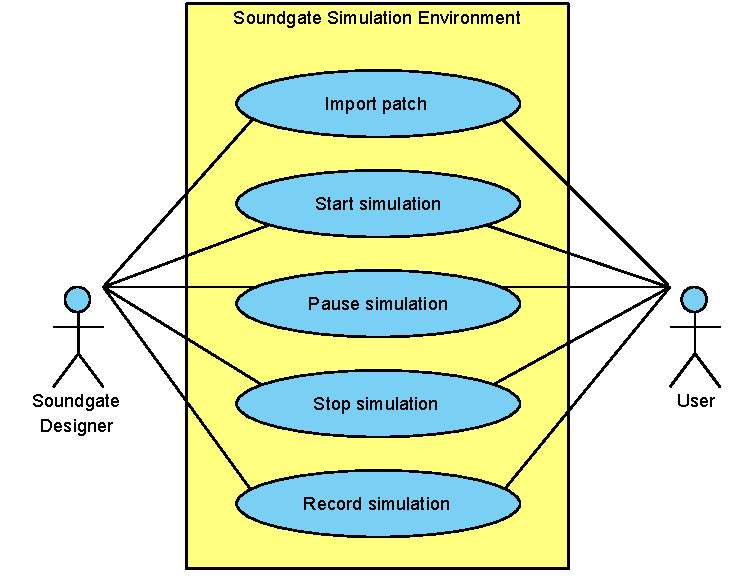
\includegraphics[width=0.90\textwidth]{images/Soundgate_Simulator.pdf}
		\caption{Use case diagram of the soundgate simulation environment}
		\label{fig:Soundgate_Simulator}
	\end{figure}

We want to develop a software simulator for a patch such the designer und the user can test the sound of the patch before putting it on the FPGA. A designer or an end-user must be able to import a patch to the simulator and to start the simulation. Then he can pause or stop the simulation. An extra feature we want to implement is that the simulation can be recorded.

\section{End-user product}

	\begin{figure}[!h]
		\centering
			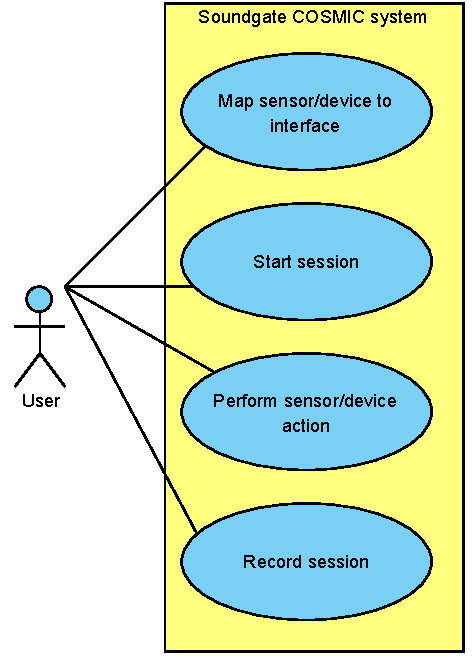
\includegraphics[width=0.90\textwidth]{images/User_View.pdf}
		\caption{Use case diagram of the soundgate user interface}
		\label{fig:Soundgate_UserInterface}
	\end{figure}
	
	As mentioned before, a patch created in the editor can be exported as XML-file which is used to generate VHDL-code. This VHDL-code is synthesized and put on a FPGA. The end-user (e.g. a musician or a performer) maps sensor values and other inputs to the interfaces defined by the designer (see ..). He starts the session by pushing a button. During the session he performs some sensor actions or actions with other devices to create input values to the system. An extra feature we want to develop is that a session can be recorded.
	
\subsection{Input}
We plan to use smartphones as sensor devices. For this purpose we want to develop a special smartphone app. Furthermore the end-user should be able to use MIDI devices.

\section{Component library}
We plan to provide following components:

\begin{itemize}
\item Generators:
\begin{itemize}
\item Sinus
\item Sawtooth
\end{itemize}

\item Filters:
\begin{itemize}
\item Ramp
\item Low pass
\item Delay
\end{itemize}

\item Arithmetic:
\begin{itemize}
\item Addition 
\item Multiplication
\item Equals
\end{itemize}

\item Mixer

\item Sources:
\begin{itemize}
\item Constant
\end{itemize}

\item Sinks:
\begin{itemize}
\item Sound output
\end{itemize}

\item MIDI: 
\begin{itemize}
\item MIDI note to frequency converter
\item MIDI scheduler
\end{itemize}

\end{itemize}